\section{电场}

\subsection{电场强度方向}

\begin{proset}
    如图，直角三角形\(\angle ABC\)处在点电荷的电场中，\(\angle B =\) \,\qty{90}{\degree}，\(A\)、\(B\)、\(C\)三点与点电荷在同一平面内，\(O\)为\(AB\)的中点，将一正的点电荷从\(A\)点沿\(AC\)移到\(C\)点，电场力一直做负功，从\(C\)点沿\(CB\)移到\(B\)点，电场力一直做正功，从\(A\)点到\(C\)点克服电场力做的功与\(C\)点到\(B\)点电场力做的功相等。下列图中箭头表示\(C\)点电场的方向，则正确的是\paren[]
    
    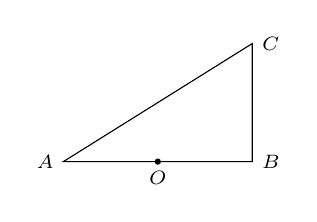
\begin{tikzpicture}[font=\scriptsize]
        \draw (0,0)node[left]{\(A\)}--(2.4,0)node[right]{\(B\)}--(2.4,1.5)node[right]{\(C\)}coordinate(c)--cycle;
        \fill (1.2,0)node[below]{\(O\)} circle(.04);
    \end{tikzpicture}

    \begin{tikzpicture}[font=\scriptsize,decoration={markings,mark=at position 0.55 with {\arrow{>}}}]
        \begin{scope}
            \draw (0,0)node[left]{\(A\)}--(2.4,0)node[right]{\(B\)}--(2.4,1.5)node[right]{\(C\)}coordinate(c)--cycle;
            \fill (1.2,0)node[above left]{\(O\)} circle(.04);
            \draw[postaction={decorate},blue] (c)--(0,0);
            \node at(1.2,-.5){A};
        \end{scope}
        \begin{scope}[xshift=3.5cm]
            \draw (0,0)node[left]{\(A\)}--(2.4,0)node[right]{\(B\)}--(2.4,1.5)node[right]{\(C\)}coordinate(c)--cycle;
            \fill (1.2,0)node[above left]{\(O\)} circle(.04);
            \draw[postaction={decorate},blue] (c)--(1.2,0);
            \node at(1.2,-.5){B};
        \end{scope}
        \begin{scope}[xshift=7cm]
            \draw (0,0)node[left]{\(A\)}--(2.4,0)node[right]{\(B\)}--(2.4,1.5)node[right]{\(C\)}coordinate(c)--cycle;
            \fill (1.2,0)node[above left]{\(O\)} circle(.04);
            \draw[postaction={decorate},blue] (c)--(1.9,0);
            \node at(1.2,-.5){C};
        \end{scope}
        \begin{scope}[xshift=10.5cm]
            \draw (0,0)node[left]{\(A\)}--(2.4,0)node[right]{\(B\)}--(2.4,1.5)node[right]{\(C\)}coordinate(c)--cycle;
            \fill (1.2,0)node[above left]{\(O\)} circle(.04);
            \draw[postaction={decorate},blue] (c)--(2.4,0);
            \node at(1.2,-.5){D};
        \end{scope}
    \end{tikzpicture}
\end{proset}
\begin{answer}
    C\quad 提示：
\end{answer}

\subsection{电势能}

\begin{proset}
    （多选）
    如图三个点电荷分别固定在边长为\(a\)的等边三角形的三个顶点上，电荷量分别为\( + q\)、\( + 2q\)、\( + 2q\)，\(O\)为三角形的中心，此时系统的电势能为\(E_0\)，已知两个带电荷量分别为\(q_1\)、\(q_2\)的点电荷组成和系统的电势能为\(\frac{kq_1q_2}{r^2}\)，\(k\)为静电常量，\(r\)为点电荷之间的距离。以下说法正确的是\paren[]

    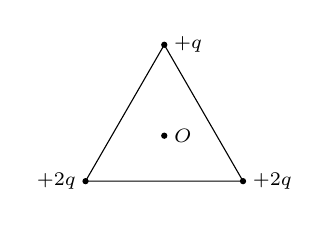
\begin{tikzpicture}[font=\scriptsize]
        \draw (0,0)coordinate(c)node[left]{\( + 2q\)}--++(60:2)coordinate(a)node[right]{\( + q\)}--++(-60:2)coordinate(b)node[right]{\( + 2q\)}--cycle;
        \foreach \c in{a,b,c}
            \fill (\c) circle(.04);
        \fill (30:{2*sqrt(3)/3}) circle(.04)node[right]{\(O\)};
    \end{tikzpicture}
    \begin{choices}
        \item \(O\)点的场强大小为\(\frac{3kq^2}{a^2}\)
        \item \(O\)点的场强大小为\(\frac{2kq^2}{2a^2}\)
        \item 若取走一个\( + 2q\)的点电荷，系统的电势能将减小\(\frac{E_0}{2}\)
        \item 若取走一个\( + 2q\)的点电荷，系统的电势能将减小\(\frac{E_0}{4}\)
    \end{choices}
\end{proset}
\begin{answer}
    AD\quad 提示：
\end{answer}